% ------------------------------------------------------------
% ------------------------------------------------------------

\section{Bluetcl Reference}
\label{tcl-commands}

Bluetcl is a Tcl extension with a collection of scripts and packages
providing an interface into the BSC view of a design.
You can execute Bluetcl commands and scripts from a
unix command line.

Bluetcl contains several layers (scripts, commands, packages) which
should be familiar to the Tcl
programmer.  You can use Bluetcl extensions within Tcl scripts.
More information on Tcl is available at \te{www.tcl.tk} or
from the many books and references written about Tcl/Tk.

% ------------------------------------------------------------

\subsection{Invoking Bluetcl}

Bluetcl commands can be run either interactively or through Tcl
scripts.  These commands load, execute, and interact with
BSC-generated  files.   As with BSC,
pre-elaboration  information is obtained
from the \te{.bo} files, and post-elaboration information is
obtained from the \te{.ba} files.  

Bluetcl commands can be invoked in the following  ways:
\begin{itemize}
\item You can invoke Bluetcl from a unix prompt by typing
\te{bluetcl}.  This command provides a Tcl shell with the Bluetcl
extensions.
\item You can write and use Tcl scripts which use Bluetcl.
For an example of a Tcl script provided with BSC, see
Section \ref{script-expandports}.
\end{itemize}

% ------------------------------------------------------------

\subsection{Packages and namespaces}
\label{packages}

Bluetcl is organized into a collection of packages, which are
described in this appendix. The major packages are:
\begin{itemize}
\item The \te{Bluetcl} package which contains the low-level commands  to  interact with Bluespec files and designs.  
\item The \te{Bluesim} package containing Bluesim command extensions.\footnote{The  {\bf\tt sim} command for interacting with
Bluesim simulation objects (\te{.so} files) is contained in both the
\te{Bluetcl} and \te{Bluesim} packages.}
\end{itemize}

All commands in the \te{Bluetcl} package are in the \te{Bluetcl}
namespace.  All commands in the \te{Bluesim} package are in the
\te{Bluesim} namespace.

When referencing a command you must specify the namespace.  Example:
\begin{verbatim}
    Bluetcl::version
\end{verbatim}
Alternately, you can import commands from a namespace.  The following example
imports all the commands in a namespace:
\begin{verbatim}
    namespace import ::Bluetcl::*
\end{verbatim}
Or you can import a single command:
\begin{verbatim}
    namespace import ::Bluetcl::schedule
\end{verbatim}

Refer to the \te{Tcl} documentation for additional information on packages
and namespaces.

% ------------------------------------------------------------

\subsection{Customizing Bluetcl}
\label{custom}
\index{.bluetclrc}

You can use Bluetcl, along with all standard Tcl constructs, to
write scripts and issue commands.
Bluetcl will source the setup
file \te{\$HOME/.bluetclrc} during initialization.  You can customize
Bluetcl by adding to the \te{.bluetclrc} file.

% The Bluetcl interpreter is
% identical to the standard Tcl interpreter with the
% following additions:
% \begin{itemize}
% \item It include the Bluetcl packages
% \item Its search paths are setup to look for other BSC
% extensions and customizations.
% \end{itemize}

The \te{namespace import} command can be put in the \te{.bluetclrc}
file, providing the command into the current namespace when the file
is sourced.  This will allow you to use just the command name in
scripts or from the command line.

% ------------------------------------------------------------

\subsection{Package command reference}

% Bluetcl is made up of  commands (or procs) to interact with
% BSC-generated files.  The  commands are organized into packages
% and namespaces, as described in Section \ref{packages}.
% The convention is to use the
% same name for both the package and the namespace.

% -------------------------

\subsubsection{Conventions}

The following conventions are used within the command reference:
\begin{tabbing}
keywordandafew     \=     \kill
{\em name} \> identifier \\
{\bf keyword} \> as is \\
$[...]$ \> optional \\
%\{...\} \> repeated\\
\end{tabbing}

When an argument (or token) contains embedded spaces, the argument may
need to be enclosed in brackets (\te{\{ \}}).
% Note: For repeated arguments (\{ \}), one or more arguments may be
% specified. If only one item is specified, no brackets (\{ \}) should
% be used.  If multiple arguments are specified the list may be
% enclosed in brackets. 

% NOTE:I need a working example.  flag show seems to use a different syntax.
% Example:
% \begin{verbatim}
%      flag show sched-dot 
% This works differently - doesn't follow syntax
%      flag show sched-dot license-type p
% \end{verbatim}

% -------------------------

\subsubsection{Bluetcl}

This sections describes the commands in the \te{Bluetcl} package.  These commands
provide a low-level interface to access BSC-specific files
(\te{.bo/.ba}) for use by Tcl programmers; they are not intended
for interactive use.  

Before using a command from the \te{Bluetcl package},  the
following Tcl command must  be executed, either in a script, 
from the command line, or in the \te{.bluetclrc} file:
\begin{verbatim}
    package require Bluetcl
\end{verbatim}

All commands in the \te{Bluetcl} package are in the  \te{Bluetcl::}
namespace.  The namespace must be referenced, as described in Section
\ref{custom}, either by using the \te{namespace import} command or by
prepending the command name with \te{Bluetcl::}.  Example:
\begin{verbatim}
    Bluetcl::bpackage list
\end{verbatim}

% -----

\subsubsubsection{Bluetcl::bpackage}
\index{bpackage@\te{bpackage} (bluetcl command)}
\index[commands]{Bluetcl!bpackage}

 Controls loading and unloading of packages
 and returns  package information. When a
package is loaded, all dependent (imported) packages are loaded as
well. 

\begin{tabular}{|p {1.8 in}| p {3.8 in}|}
\hline
\hline
{\bf bpackage} {\bf load} {\em packname} [{\em packname ...}]& Reads in the \te{.bo} package and all
imported packages. Packages are searched in the standard bsc way, via
the \te{-p} flag. Returns a list of all packages which are loaded.
One or more package names can be provided.\\
\hline
{\bf bpackage} {\bf  list}&Returns the list of packages which are loaded.\\
\hline
{\bf bpackage} {\bf  clear}&Clear all currently loaded packages.\\
\hline
{\bf bpackage} {\bf  depend} & Returns package dependencies of all currently loaded
packages. \\
\hline
{\bf bpackage} {\bf  search} {\em regex}& Searches packages for names matching a
regular expression. \\
\hline
{\bf bpackage} {\bf  types} {\em packname}& Returns a list of type names found
in the package.\\
\hline
\hline
\end{tabular}

% -----

% \subsubsubsection{Bluetcl::browseinst}
% \index{browseinst@\te{browseinst} (bluetcl command)}
% \index[commands]{Bluetcl!browseinst}

% Returns information on instantiations in the current (post
% elaboration) module hierarchy.

% \begin{tabular}{|p {1.8 in}| p {3.8 in}|}
% \hline
% \hline
% {\bf browseinst} {\bf  list} {\em key}& Returns a list specifying the
% children of the \te{inst} with \te{key} {\em key}. Each list item
% specifies the \te{key} of the child, as well as its type (i.e. does it
% corresponds to a rule, a synthesized module instantiation, or a BSV
% module instantiation).\\
% \hline
% {\bf browseinst} {\bf  detail} {\em key}& Returns of list information
% about the \te{inst} with \te{key} {\em key}. Information includes
% name, full instantiation path, and associated interface. \\
% \hline
% {\bf browseinst} {\bf  search} {\em regex}& Returns a list. Each list
% item specifies an \te{inst} that matches the specified regular
% expression, {\em regex}. Each list item specifies the \te{key} of the
% \te{inst}, as well as its type (i.e. does it corresponds to a rule, a
% synthesized module instantiation, or a BSV module instantiation). \\
% \hline
% \hline
% \end{tabular}

% -----

\subsubsubsection{Bluetcl::defs}
\index{defs@\te{defs} (bluetcl command)}
\index[commands]{Bluetcl!defs}

Returns a list of the components defined in a package.  Components
returned include types, synthesized modules, and functions.

\begin{tabular}{|p {1.8 in}| p {3.8 in}|}
\hline
\hline
{\bf defs} {\bf  all} {\em packname}& Returns a list of all components which
are defined in the package. \\
\hline
{\bf defs} {\bf  type} {\em packname}&
Returns a list of all types which are defined in the package.\\
\hline
{\bf defs} {\bf  module} {\em packname}&
Returns a list of all module names defined in the package which are marked
synthesize. \\
\hline
{\bf defs} {\bf  func} {\em packname}&
Returns a tagged structure list of all functions which are defined in the package.
\\
\hline
\hline
\end{tabular}

% -----

\subsubsubsection{Bluetcl::flags}
\index{flags@\te{flags} (bluetcl command)}
\index[commands]{Bluetcl!flags}

Returns or sets the status of flags used by BSC.

\begin{tabular}{|p {1.8 in}| p {3.8 in}|}
\hline
\hline
{\bf flags} {\bf  show} {\em flagname} [{\em flagname ...}] &Show the
value of the specified flags.  One ore more flag names can be provided.\\
\hline
{\bf flags} {\bf  set} {\em flagname} {\em value} [{\em flagname}
{\em value} ...] & Set the flags to the value provided. Multiple flags
may be set in a single command.  \\
\hline
\hline
\end{tabular}

Note: Values enclosed in brackets define a single token. 
For example,  setting the value of the flag \te{-verilog-filter} with
embedded spaces:

\begin{verbatim}
Bluetcl::flags set -verilog-filter {sed -e -e 's/XX/SS/'}
\end{verbatim}

% -----

\subsubsubsection{Bluetcl::help}
\index{help@\te{help} (bluetcl command)} 
\index[commands]{Bluetcl!help}

Help with no arguments will list all available help topics.
Optionally, an argument can be provided to get help on a specific topic.
Also, 'help list' will return a string listing the names of all commands.

\begin{tabular}{|p {1.8 in}| p {3.8 in}|}
\hline
\hline
{\bf help} & Returns a list of all help topics.\\
\hline
{\bf help} {\bf  list} & Returns a string listing the name of all commands\\ 
\hline
{\bf help} {\em  command} & Returns help for the specified command. \\ 
\hline
\hline
\end{tabular}

% -----

\subsubsubsection{Bluetcl::module}
\index{module@\te{module} (bluetcl command)}
\index[commands]{Bluetcl!module}

Returns information on synthesized (post elaboration) modules.

\begin{tabular}{|p {1.8 in}| p {3.8 in}|}
\hline
\hline
{\bf module} {\bf  load} {\em modname}& Loads the module and all
instantiated submodules into Bluetcl's workspace. Returns a list of the
modules loaded. \\
\hline
{\bf module} {\bf  clear} &Clear all loaded modules \\
\hline
{\bf module}  {\bf submods} {\em modname}& Returns a 3-tuple. The first
element of the tuple is a tag (primitive or user), the second is a
list of pairs contain the synthesized submodule name and its interface
type. The third element  is a list of function which have
not been in-lined.\\
\hline
{\bf module} {\bf  rules} {\em modname}&
Returns a list of rule names in the module.\\
\hline
{\bf module} {\bf  ifc} {\em modname} &
Returns a list of interface types in the module.\\
\hline
{\bf module} {\bf  methods} {\em modname}& Returns a list of the  flattened methods
in the module. \\
\hline
{\bf module}  {\bf  ports} {\em modname}& Returns a list of  the ports in the module. \\
\hline
{\bf module} {\bf porttypes} {\em modname}& Returns a list of  the types of the ports in
the module. \\
\hline
{\bf module} {\bf list}& Returns a list of all loaded modules.\\
\hline
\hline
\end{tabular}

% -----

\subsubsubsection{Bluetcl::rule}
\index{rule@\te{rule} (bluetcl command)}
\index[commands]{Bluetcl!rule}
Returns information about rules in a post elaboration module.

\begin{tabular}{|p {2.0 in}| p {3.6 in}|}
\hline
\hline
{\bf rule} {\bf  rel} {\em modname rule1 rule2}& Shows the relationship
between two rules in the module.\\
\hline
{\bf rule} {\bf  full} {\em modname rule}&
Returns a tagged structure detailing the rules position, 
predicates expression,  attributes and  method calls. \\
\hline
\hline
\end{tabular}

% -----

\subsubsubsection{Bluetcl::schedule}
\index{schedule@\te{schedule} (bluetcl command)}
\index[commands]{Bluetcl!schedule}

Returns scheduling information for a synthesized module.  The
\te{schedule}  command
requires a subcommand and the module name.

\begin{tabular}{|p {2.1 in}| p {3.5 in}|}
\hline
\hline
{\bf schedule} {\bf  execution} {\em modname}&Returns a list of rule/method
names in execution order.  For example, if \te{r1} fires after
\te{r2}, then the output would be: \te{RL\_r1 RL\_r2}.\\
\hline
{\bf schedule} {\bf  methodinfo} {\em modname}&Returns scheduling
relationships between all pairs of methods.\\
\hline
{\bf schedule} {\bf  pathinfo} {\em modname}&Returns a list of combinational
paths through the module.  Each element is a list of two elements: a
list of inputs and an output that they connect to.\\
\hline
{\bf schedule} {\bf  urgency} {\em modname}&Returns a list of lists, one for
each rule/method, in urgency order.  Each lists contains two elements:
the rule name and a list of rules which would block that rule from firing.\\
\hline
{\bf schedule} {\bf  warnings} {\em modname}&Returns a list of scheduling
warnings.  The result is a list of three elements: the position
of the warning, the tag for the warning, and the complete warning message.  \\
\hline
\hline
\end{tabular}

% -----

\subsubsubsection{Bluetcl::sim}
\index{sim@\te{sim} (bluetcl command)}
\label{bluetcl-sim}
\index[commands]{Bluetcl!sim}

 Controls all aspects of loading, executing and interacting
with a Bluesim simulation object.  These commands are used when
running Bluesim interactively, as described in section \ref {bluesim-interactive}. 

This command is also provided in the \te{Bluesim} package.  See section
\ref{bluesim-sim} for the complete definition.

% -----

\subsubsubsection{Bluetcl::submodule}
\index{submodule@\te{submodule} (bluetcl command)}
\index[commands]{Bluetcl!submodule}

Returns information about each submodule and
which rules use the methods of the submodule.

\begin{tabular}{|p {1.8 in}| p {3.8 in}|}
\hline
\hline
{\bf submodule} {\bf  full} {\em modname}& Returns information about each
submodule in the specified module and the rules which use the methods
of the submodule. \\
\hline
\hline
\end{tabular}

% -----

\subsubsubsection{Bluetcl::type}
\index{type@\te{type} (bluetcl command)}
\index[commands]{Bluetcl!type}
 Finds and returns type information.

\begin{tabular}{|p {1.8 in}| p {3.8 in}|}
\hline
\hline
{\bf type} {\bf  constr} {\em typename}& Shows the type constructor for
the provided type name. The type constructor is the type arguments
needed for the type. Returns an error if the typename is not found in
any of the loaded packages. \\ 
\hline
{\bf type} {\bf full} {\em typeconstructor}&Returns a tagged structure
based on the type constructor argument. The type constructor provided
must be fully qualified. \\
\hline
\hline
\end{tabular}

% -----

\subsubsubsection{Bluetcl::version}
\index{version@\te{version} (bluetcl command)}
\index[commands]{Bluetcl!version}

Returns the current compiler version

\begin{tabular}{|p {1.8 in}| p {3.8 in}|}
\hline
\hline
{\bf version} &Returns a list of 3 items: the compiler version, the
version date, and the build  version. The compiler version is
provided  in year-month-(annotation) format. \\
\hline
\hline
\end{tabular}

% -------------------------

\subsubsection{Bluesim}

The Bluesim package contains the \te{sim} command which controls
Bluesim interactive mode.  This command is also found in the
\te{Bluetcl} package.

Before using a command from the Bluesim package,  the
following Tcl command must  be executed, either in a script, 
from the command line, or in the \te{.bluetclrc} file:
\begin{verbatim}
    package require Bluesim
\end{verbatim}

All commands in the \te{Bluesim} package are in the  \te{Bluesim::}
namespace.  The namespace must be referenced, as described in Section
\ref{custom}, either by using the \te{namespace import} command or by
prepending the command name with \te{Bluesim::}.  Example:
\begin{verbatim}
    Bluesim::sim clock
\end{verbatim}

% -----

\subsubsubsection{sim}
\index{sim@\te{sim} (bluesim command)}
\label{bluesim-sim}
\index[commands]{Bluesim!sim}

 Controls all aspects of loading, executing and interacting
with a Bluesim simulation object.  These commands are used when
running Bluesim interactively, as described in section \ref {bluesim-interactive}. 
This command is also provided in the \te{Bluetcl} package (\ref{bluetcl-sim}).

\begin{tabular}{|p {1.8 in}| p {3.8 in}|}
\hline
\hline
{\bf sim} {\bf arg} {\em string} &Set a simulation plus-arg. Adds the supplied
{\em string} to the end of the list of plusargs searched by the
\te{\$test\$plusargs} system task. \\
\hline
\end{tabular}

\begin{tabular}{|p {1.8 in}| p {3.8 in}|}
\hline
{\bf sim} {\bf  cd} [{\em path}]&Change location in hierarchy.   The
path must consist of a sequence of instance names separated by a
period (\te{.}).  A path which begins with a \te{.} is an absolute
path from the top of the hierarchy, but one which does not begin with
a \te{.} is relative to the current location.  No provided {\em path} will
return the user to the uppermost point in the hierarchy.\\
\hline
\end{tabular}

\begin{tabular}{|p {1.8 in}| p {3.8 in}|}
\hline
{\bf sim} {\bf  clock} & Returns a
list containing a clock description for each currently defined clock.\\
\hline
{\bf sim} {\bf  clock} [{\em name}]& Select the named clock, make it
the active clock.\\
\hline
\end{tabular}

\begin{tabular}{|p {1.8 in}| p {3.8 in}|}
\hline
{\bf sim} {\bf describe} {\em handle}&Describe the object to which a symbol
handle refers.\\
\hline
\end{tabular}

\begin{tabular}{|p {1.8 in}| p {3.8 in}|}
\hline
{\bf sim} {\bf  get} {\em handle}&Returns the simulation value for
the object with the provided {\em handle}.  The value is returned as a
sized hexadecimal number. \\
\hline
\end{tabular}

\begin{tabular}{|p {1.8 in}| p {3.8 in}|}
\hline
{\bf sim} {\bf  getrange} {\em handle addr}&Get simulation values from a range.  \\
\hline
\end{tabular}

\begin{tabular}{|p {1.8 in}| p {3.8 in}|}
\hline
{\bf sim} {\bf   load} {\em model} &Load a bluesim model object.\\
\hline
\end{tabular}

\begin{tabular}{|p {1.8 in}| p {3.8 in}|}
\hline
{\bf sim} {\bf   lookup} {\em pattern} [{\em root}]&Lookup symbol
handles.  Returns a handle for every simulation object which matches
the {\em pattern}.   \\
\hline
\end{tabular}

\begin{tabular}{|p {1.8 in}| p {3.8 in}|}
\hline
{\bf sim} {\bf   ls} {\em pattern} *&List the sub-instances, rules and
values at that level of the hierarchy.  If a {\em pattern} is
provided, it controls which names are listed.  No pattern is
equivalent to \te{sim ls *}.  \\
\hline
\end{tabular}


\begin{tabular}{|p {1.8 in}| p {3.8 in}|}
\hline
{\bf sim} {\bf  nextedge }&Advance simulation to the next clock edge in any domain.\\
\hline
\end{tabular}

\begin{tabular}{|p {1.8 in}| p {3.8 in}|}
\hline
{\bf sim} {\bf   pwd}&Print current location in hierarchy.\\ 
\hline
\end{tabular}

\begin{tabular}{|p {1.8 in}| p {3.8 in}|}
\hline
{\bf sim} {\bf  run} [{\bf async}]&Run simulation to completion.  The
keyword \te{async} cause the command to return immediately so that
additional commands can be processed while the simulation continues to
run asynchronously.\\  
\hline
\end{tabular}

\begin{tabular}{|p {1.8 in}| p {3.8 in}|}
\hline
{\bf sim} {\bf  runto} {\em time} [{\bf async}]&Run simulation to a
given time. The
keyword \te{async} cause the command to return immediately so that
additional commands can be processed while the simulation continues to
run asynchronously.\\  
\hline
\end{tabular}

\begin{tabular}{|p {1.8 in}| p {3.8 in}|}
\hline
{\bf sim} {\bf  step} [{\em cycles}] [{\bf async}]&Advance simulation
a given number of cycles. The
keyword \te{async} cause the command to return immediately so that
additional commands can be processed while the simulation continues to
run asynchronously. \\
\hline
\end{tabular}

\begin{tabular}{|p {1.8 in}| p {3.8 in}|}
\hline
{\bf sim} {\bf  stop}&:stop the simulation at the end of the currently
executing simulation cycle.\\
\hline
\end{tabular}

\begin{tabular}{|p {1.8 in}| p {3.8 in}|}
\hline
{\bf sim} {\bf  sync}&Wait for simulation to complete normally before returning\\  
\hline
\end{tabular}

 \begin{tabular}{|p {1.8 in}| p {3.8 in}|}
\hline
{\bf sim} {\bf  time}&Display current simulation time.\\
\hline
\end{tabular}

\begin{tabular}{|p {1.8 in}| p {3.8 in}|}
\hline
{\bf sim} {\bf  unload}&Unload the current bluesim model.\\
\hline
\end{tabular}

\begin{tabular}{|p {1.8 in}| p {3.8 in}|}
\hline
{\bf sim} {\bf  up} [{\em N}]&Move up the module hierarchy into the
parents of the current directory.  It will move up \te{N} levels if
{N} is provided. \\  
\hline
\end{tabular}

\begin{tabular}{|p {1.8 in}| p {3.8 in}|}
\hline
{\bf sim} {\bf  vcd} [{\bf on} $\mid$ {\bf off} $\mid$ {\em file}]&Control
dumping waveforms to a VCD file named {\em file}. If no file name is
provided, it will use the default file \te{dump.vcd}.\\
\hline
\end{tabular}

\begin{tabular}{|p {1.8 in}| p {3.8 in}|}
\hline
{\bf sim} {\bf   version}&Show Bluesim model version information.\\  
\hline
\hline
\end{tabular}

% -------------------------

\subsubsection{InstSynth}
The \te{InstSynth} package contains scripts to generate instance
specific synthesis in Bluespec SystemVerilog.  These scripts use
Bluespec's typeclass and overloading to match a module's instantiation
with a specific instance which may instantiate a synthesized module.

When using any of the commands in the \te{InstSynth} package, the
package must be loaded first.

\begin{verbatim}
     package require InstSynth
\end{verbatim} 


The \te{InstSynth} package contains the commands 
\te{genTypeClass}, \te{genSpecificInst}, and \te{genSynthMod}.

% \paragraph{genTypeClass}
% Creates an include file for a package.

% \begin{tabular}{|p {5.8 in}|}
% \hline
% \hline
% \\
% {\bf genTypeClass} {\em packname} \{{\em modname}\}\\
% \\
% \hline
% Creates an include file for a package containing  a
%  typeclass for overloading 
% of a module and a default instance for the module.  Multiple modules
%  within the same package can be specified in a single command. \\
% \hline
% \hline
% \end{tabular}

% \paragraph{genSpecificInst}
% Modifies the include file generated by the \te{genTypeClass} proc to
% add an instance for each missing type.


% \begin{tabular}{|p {5.8 in}|}
% \hline
% \hline
% \\
% {\bf genSpecificInst} {\em packname} {\em modname} {\em type} \\
% \\
% \hline
%  Modifies the {\em packname}\te{.include.bsv} file with an instance for each missing type.\\
% \hline
% \hline
% \end{tabular}


% \begin{tabular}{|p {5.8 in}|}
% \hline
% \hline
% \\
% {\bf genSynthMod} {\em packname} {\em modname} {\em type}\\
% \\
% \hline
% Generates a synthesize module wrapper for a given module and type
% within a package.   The generated module is returned as a string from
% this function.\\
% \hline
% \hline
% \end{tabular}




% \begin{tabular}{|p {2.2 in}| p {3.4 in}|}
% \hline
% \hline
% {\bf genSpecificInst} {\em packname} {\em modname} {\em type} & Modifies the {\em packname}\te{.include.bsv} file with an instance for each missing type.\\
% \hline
% \hline
% \end{tabular}



\begin{tabular}{|p {1.4 in}| p {4 in}|}
\hline
% {\bf Proc}&{\bf Usage} \\
% \cline{2-2}
% &{\bf Description}\\
\multicolumn{2}{|c|}{}\\
\multicolumn{2}{|c|}{\bf InstSynth Commands}\\
\hline
\hline
&\\
\te{genTypeClass}&{\bf genTypeClass} {\em packname} \{{\em modname}\}\\
\cline{2-2}
&\\
 &Creates an include file for a package containing  a
 typeclass for overloading 
of a module and a default instance for the module.  Multiple modules
 within the same package can be specified in a single command. \\ 
\hline
&\\
\te{genSpecificInst} &{\bf genSpecificInst} {\em packname} {\em modname} {\em type}  \\
\cline{2-2}
&\\
&Modifies the {\em packname}\te{.include.bsv} file with an instance for each missing type.\\
\hline
&\\
\te{genSynthMod}&{\bf genSynthMod} {\em packname} {\em modname} {\em type}\\
\cline{2-2}
&\\
&Generates a synthesize module wrapper for a given module and type
within a package.   The generated module is returned as a string from
this function.\\
\hline
\hline
\end{tabular}


{\bf Example using InstSynth.tcl to generate instance
specific synthesis modules}

Overview:
This example demonstrates how to use the \te{InstSynth.tcl} package to use
Bluespec's  typeclass and overloading to
match a module's instantiation with a specific instance to
instantiate a synthesized module.

The example is composed of three \te{.bsv} files: \te{m1.bsv} which
contains  the
module definition for \te{mkM1}, \te{m2.bsv} which contains the module
definition for \te{mkM2} and instantiates multiple instances of
\te{mkM1}, and \te{Top.bsv} containing the testbench \te{mkTb}.  The
two modules \te{mkM1} and \te{mkM2} are polymorphic.  The testbench
\te{mkTb} instantiates \te{mkM2} and is not polymorphic.  

The polymorphic modules are instantiated in the hierarchy as shown in
figure \ref{hierarchy}.

\begin{figure}[ht]
\begin{center}
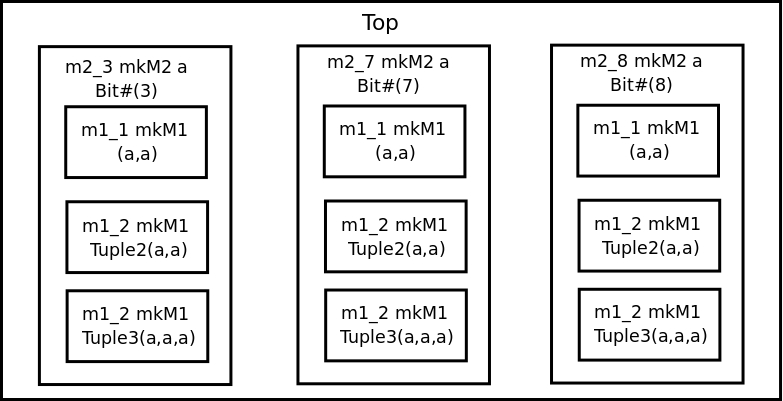
\includegraphics[width = 4 in]{figures/hierarchy}
\caption{Example Module Hierarchy}
\label{hierarchy}
\end{center}
\end{figure}

{\bf Steps for using InstSynth}
 \begin{enumerate}

 \item  Compile your design with bsc as normal, creating the
 \te{.bo} files.

 \item Generate typeclass and default instances for modules with
 the \te{genTypeClass} command, specifying the packages and modules for 
 instance specific synthesis.   The \te{genTypeClass} command will generate
 an include file (\te{<package>}\te{.include.bsv}) for each package.

  The include file will contain  a type class (named
   \te{MakeInst\_<module>}) for each module and a general
   catch-all   instance of that type class.   

   The type class contains one method, which is a module constructor.
   The method is named \te{<module>\_Synth} and has the same arguments as the
   general polymorphic module.  The instance of  this type class is
   a thin wrapper which instantiates the polymorphic module and prints
   a message about the type which is synthesized.

 Example of the include file for \te{m1.bsv} (\te{m1.include.bsv})
 after this step:
 \begin{verbatim}
 typeclass MakeInst_mkM1 #(type ifc_t);
     module mkM1_Synth ( ifc_t ifc) ;
 endtypeclass

 instance MakeInst_mkM1 #(  ClientServer::Server#(a, a) )
     provisos (Bits#(a, sa)) ;

     module mkM1_Synth ( ClientServer::Server#(a, a) ifc) ;
         let _i <- mkM1  ;
         messageM ("No concrete definition of mkM1 for type " +
                    (printType (typeOf (_i))));
         messageM ("Execute: InstSynth::genSpecificInst m1 mkM1 {" +

                     " {" + (printType (typeOf(asIfc (_i)))) + "}" 
                     + " }"  );
         return _i ;
     endmodule
 endinstance
 \end{verbatim}


 \item Manually edit the  \te{.bsv} file to  include the generated file.
 For example, add the line \te{`include "}\te{<package>}\te{.include.bsv"} at the
 bottom of the file for \te{<package>}.  In this example, you would add the line
 \te{`include "m1.include.bsv"} to the file \te{m1.bsv}.

 \item Manually edit the \te{.bsv} file to change the module
 constructor from \te{<module>} to \te{<module\_Synth>} at each point you
 would like an instance synthesized.
 In this example, change  \te{mkM1} to \te{mkM1\_Synth} in the
 \te{m2.bsv} file, and change \te{mkM2} to \te{mkM2\_Synth} in the
 \te{Top.bsv} file where you want to synthesize an instance.


 \item Compile the design again with bsc.   The compile will generate messages
listing missing instances along with the \te{genSpecificInst} command to
 create each missing instance.   Execute the commands 
one at a time to generate an instance for each missing type. 

The \te{genSpecificInst} command will modify the \te{include.bsv} files,
adding the instances.  For example, in this step, the following lines
are added to the \te{m1.include.bsv} file to resolve the
\te{Server\#(a,a)} type.  

\begin{verbatim}
module mkM1__ClientServer_Server_Bit_3_Bit_3_(
                              ClientServer::Server#(Bit#(3), Bit#(3)) ifc ) ;
    let _i <- mkM1  ;
    return _i ;
endmodule

instance MakeInst_mkM1 #( ClientServer::Server#(Bit#(3), Bit#(3)) ) ;
    module mkM1_Synth ( ClientServer::Server#(Bit#(3), Bit#(3)) ifc );
        let _i <- mkM1__ClientServer_Server_Bit_3_Bit_3_  ;
        messageM("Using mkM1__ClientServer_Server_Bit_3_Bit_3_ for mkM1 of
                type: " +
                  (printType (typeOf (_i))));
         return _i ;
     endmodule
endinstance
\end{verbatim}

Note that the code added in this step does not add to or change the
behavior of the design.  Only the additional hierarchy is added.

\item Add provisos to the polymorphic modules to avoid early binding
of the module.  Otherwise compiling at this point will not show the
specific instances because the instance of the \te{\_Synth} is bound
before the specific type of the module is known. In this example,
\te{mkM1\_Synth} would be  bound
before  the specific type of \te{mkM2} is known.  To fix this,  
provisos  are added to the
polymorphic module \te{mkM2}.  The module \te{mkM2} has three
instantiations of \te{mkM1}, therefore a proviso for each
instantiation is  added.

\begin{verbatim}
module mkM2 (Server#(a,a)) provisos (Bits#(a,sa) 
                     ,MakeInst_mkM1#(Server#(a,a))
                     ,MakeInst_mkM1#(Server#(Tuple2#(a,a),Tuple2#(a,a)))
                     ,MakeInst_mkM1#(Server#(Tuple3#(a,a,a),Tuple3#(a,a,a)))
                     );

\end{verbatim} 

\item Compile with bsc again. 

\item Continue  until there are no missing instance messages.   A
Verilog file will be created for each synthesized module instance.

\end{enumerate}


{\bf SynthInst Example Files}
\label{poly-example}

{\bf m1.bsv}: Module \te{mkM1} is defined in the package (file) \te{m1.bsv}:

\begin{verbatim}
   import ClientServer :: *;
   import GetPut :: *;
   import FIFOF :: * ;

   module mkM1 (Server#(a,a))    provisos (Bits#(a,sa));
      FIFOF#(a) fifo <- mkFIFOF;

      interface request = toPut (fifo);
      interface response = toGet (fifo);
   endmodule
\end{verbatim}

{\bf m2.bsv}: Module \te{mkM2} is defined in the package \te{m2.bsv}.  Note that
there are three instantiations of \te{mkM1}.  You can choose to
synthesize any or all of the instances.

\begin{verbatim}
   import FIFO::*;
   import GetPut::*;
   import ClientServer::*;
   import m1 :: *;

   module mkM2 (Server#(a,a))    provisos (Bits#(a,sa)
      Server#(a,a) m1_1 <- mkM1;
      Server#(Tuple2#(a,a),Tuple2#(a,a)) m1_2 <- mkM1;
      Server#(Tuple3#(a,a,a),Tuple3#(a,a,a)) m1_3 <- mkM1;

      rule r0;
         let { x1,x2 } <- m1_2.response.get();
         m1_3.request.put (tuple3 (x1,x2,x2));
      endrule

      interface Put request;
         method Action put (a x);
            m1_2.request.put (tuple2(x,x));
         endmethod
      endinterface

      interface Get response;
         method ActionValue#(a) get ();
            let { y1,y2,y3 } <- m1_3.response.get();
            return (y1);
         endmethod
      endinterface
   endmodule
\end{verbatim}

{\bf Top.bsv}: The testbench is contained in the file \te{Top.bsv}
\begin{verbatim}
   import ClientServer :: *;
   import GetPut :: *;
   import m2 :: *; 
   
   (* synthesize *)
   module mkTb (Empty);
      Reg#(int) cycle <- mkReg (0);
   
      Server#(Bit#(3), Bit#(3)) m2_3 <- mkM2;
      Server#(Bit#(7), Bit#(7)) m2_6 <- mkM2;
      Server#(Bit#(8), Bit#(8)) m2_8 <- mkM2;
   
      rule r1;
         $display ("%0d: r1: put (%0d)", cycle, cycle);
         m2_3.request.put (truncate (pack (cycle)));
         m2_6.request.put (truncate (pack (cycle)));
         cycle <= cycle + 1;
         if (cycle > 8) $finish(0);
      endrule
   
      rule r2;
         let x_3 <- m2_3.response.get ();
         let x_6 <- m2_6.response.get ();
         $display ("%0d: r2: %0d,%0d <= get", cycle, x_3, x_6);
      endrule
   endmodule
\end{verbatim}

% {\bf Example: Using genSynthMod}

% The proc \te{genSynthMod} generates 

% \begin{verbatim}
% import FIFO::*;
% import GetPut::*;
% import ClientServer::*;

% import m1 :: *;
% module mkM2 (Server#(a,a))    provisos (Bits#(a,sa)
%                                         );

%    Server#(a,a) m1_1 <- mkM1;
%    Server#(Tuple2#(a,a),Tuple2#(a,a)) m1_2 <- mkM1;

%    Server#(Tuple3#(a,a,a),Tuple3#(a,a,a)) m1_3 <- mkM1;

%    rule r0;
%       let { x1,x2 } <- m1_2.response.get();
%       m1_3.request.put (tuple3 (x1,x2,x2));
%    endrule

%    interface Put request;
%       method Action put (a x);
%          m1_2.request.put (tuple2(x,x));
%       endmethod
%    endinterface

%    interface Get response;
%       method ActionValue#(a) get ();
%          let { y1,y2,y3 } <- m1_3.response.get();
%          return (y1);
%       endmethod
%    endinterface
% endmodule
% \end{verbatim}

% Given the file m2.bsv, above, and apply \te{genSynthMod}:
% \begin{verbatim}
% genSynthMod m2 mkM2 Server#(a,a) 
% \end{verbatim}

% The result is:

% \begin{verbatim}
% module mkM2__Server_a_a_ ( Server#(a,a) ifc ) ;
%     let _i <- mkM2  ;
%     return _i ;
% endmodule
% \end{verbatim}

% ------------------------------------------------------------

\subsection{Bluetcl Scripts}
Scripts are self-contained commands you run from a shell.  A Tcl
script may be include any combination of Bluetcl and Tcl commands. 

The scripts described in this section are provided with BSC in the
\te{\$BLUESPECDIR/tcllib/bluespec} directory.
To execute a script, type the fully qualified script name.  For
example, to execute the \te{expandPorts} script from a command prompt you would type:
\begin{verbatim}
    $BLUESPECDIR/tcllib/bluespec/expandPorts.tcl
\end{verbatim}

If you are already in a Tcl shell, type  \te{exec} before the script name:
\begin{verbatim}
    exec $BLUESPECDIR/tcllib/bluespec/expandPorts.tcl
\end{verbatim}

% -------------------------

\subsubsection{expandPorts}
\label{script-expandports}

Script to create a Verilog wrapper file which expands structures into
separate Verilog ports.

% -----

\subsubsubsection{Usage:}

{\bf expandPorts.tcl} \{options\} {\em packname} {\em modname}
{\em module.v}

\begin{tabular}{|p {1.8 in}| p {3.8 in}|}
\hline
\hline
options &Optional command line switches: \\
{\bf -p} {\em path}& path, if supplied to the bsc command\\
{\bf -verilog}& compile to verilog (default)\\
{\bf -sim}& compile to bluesim\\
{\bf -include} {\em outfile} &output file for \te{include.vh}\\
{\bf -wrapper} {\em outfile}&output file for \te{wrapper.v}\\
{\bf -rename file.tcl} & Tcl script creating rename pin structure\\
{\bf -makerename}&Create empty \te{.rename.tcl} file to edit for
\te{-rename}\\
{\bf -interface} {\em name}& Interface to expand - defaults to
package name ({\em packname})\\
\hline
{\em packname}& Name of the input \te{.bo} file.\\
\hline
{\em modname} & Name of the top level module.\\
\hline
{\em module.v}& bsc generated Verilog (\te{.v}) file for the module
being wrapped.\\
\hline
\hline
\end{tabular}

% ------------------------------------------------------------
% ------------------------------------------------------------
